\documentclass{article}

% Add search paths for input files
\makeatletter
\def\input@path{{../}{../../}{../texinputs/}}
\makeatother

\usepackage{amsmath}
\usepackage{framed}

%\usepackage{layout}
%\usepackage{showframe}
%%
%% Default settings for artisynth
%%
\NeedsTeXFormat{LaTeX2e}
%%\ProvidesPackage{artisynthDoc}[2012/04/05]

\usepackage[T1]{fontenc}
\usepackage[latin1]{inputenc}
\usepackage{listings}
\usepackage{makeidx}
\usepackage{latexml}
\usepackage{graphicx}
\usepackage{framed}
\usepackage{booktabs}
\usepackage{color}

\newcommand{\pubdate}{\today}
\newcommand{\setpubdate}[1]{\renewcommand{\pubdate}{#1}}
\newcommand{\code}[1]{{\tt #1}}

\iflatexml
\usepackage{hyperref}
\setlength\parindent{0pt} 
\else
%% then we are making a PDF, so include things that LaTeXML can't handle: 
%% docbook style, \RaggedRight
\usepackage{ifxetex}
\usepackage{xstring}
\usepackage{pslatex} % fixes fonts; in particular sets a better-fitting \tt font

\usepackage[most]{tcolorbox}
\definecolor{shadecolor}{rgb}{0.95,0.95,0.95}
\tcbset{
    frame code={}
    center title,
    left=0pt,
    right=0pt,
    top=0pt,
    bottom=0pt,
    colback=shadecolor,
    colframe=white,
    width=\dimexpr\textwidth\relax,
    enlarge left by=0mm,
    boxsep=0pt,
    arc=0pt,outer arc=0pt,
}%

\usepackage[A4]{artisynth_papersize}
%\usepackage[letter]{artisynth_papersize}
\usepackage[hyperlink]{asciidoc-dblatex} 

%\usepackage{verbatim}
\usepackage{ragged2e}
\setlength{\RaggedRightRightskip}{0pt plus 4em}
\RaggedRight
\renewcommand{\DBKpubdate}{\pubdate}
\renewcommand{\DBKreleaseinfo}{}
\fi

% set hypertext links to be dark blue:
\definecolor{darkblue}{rgb}{0,0,0.8}
\definecolor{sidebar}{rgb}{0.5,0.5,0.7}
\hypersetup{colorlinks=true,urlcolor=darkblue,linkcolor=darkblue,breaklinks=true}

%%%%%%%%%%%%%%%%%%%%%%%%%%%%%%%%%%%%%%%%%%%%%%%%%%%%%%%%%%%%%%%%%%%%%%%%%%%%%
%
% Define macros for handling javadoc class and method references
%
%%%%%%%%%%%%%%%%%%%%%%%%%%%%%%%%%%%%%%%%%%%%%%%%%%%%%%%%%%%%%%%%%%%%%%%%%%%%%
\makeatletter

% macro to enable line break if inside a PDF file
\def\pdfbreak{\iflatexml\else\\\fi}

% code inspired by http://stackoverflow.com/questions/2457780/latex-apply-an-operation-to-every-character-in-a-string
\def\removeargs #1{\doremoveargs#1$\wholeString\unskip}
\def\doremoveargs#1#2\wholeString{\if#1$%
\else\if#1({()}\else{#1}\taketherest#2\fi\fi}
\def\taketherest#1\fi
{\fi \doremoveargs#1\wholeString}

% Note: still doesn't work properly when called on macro output ...
% i.e., \dottoslash{\concatnames{model}{base}{foo}} fails 
\def\dottoslash #1{\dodottoslash#1$\wholeString\unskip}
\def\dodottoslash#1#2\wholeString{\if#1$%
\else\if#1.{/}\else{#1}\fi\dottaketherest#2\fi}
\def\dottaketherest#1\fi{\fi \dodottoslash#1\wholeString}

\def\hashtodot #1{\dohashtodot#1$\wholeString\unskip}
\def\dohashtodot#1#2\wholeString{\if#1$X%
\else\if#1\#{.}\else{#1}\fi\hashtaketherest#2\fi}
\def\hashtaketherest#1\fi{\fi \dohashtodot#1\wholeString}

%\dollartodot{#1} does the same thing as \StrSubstitute[0]{#1}{\$}{.}
% from the packahe xstring. We define \dollartodot instead because
% LaTeXML does not implement xstring.
%
% Note that for the substituion to work, we need \ifx instead of \if,
% since otherwise escaped characters won't work properly:
% if #1 = \$, then \if#1* seems to compare '\' and '$' (and output '*'),
% rather than comparing '$' to '*'
\def\dollartodot #1{\dodollartodot#1*\wholeString\unskip}
\def\dodollartodot#1#2\wholeString{\ifx#1*%
\else \ifx#1\${.}\else{#1}\fi\dollartaketherest#2\fi}
\def\dollartaketherest#1\fi{\fi \dodollartodot#1\wholeString}

% concatenates up to three class/method names together, adding '.' characters
% between them. The first and/or second argument may be empty, in which case
% the '.' is omitted. To check to see if these arguments are empty, we
% use a contruction '\if#1@@', which will return true iff #1 is empty
% (on the assumption that #1 will not contain a '@' character).
\def\concatnames
#1#2#3{\if#1@@\if#2@@#3\else #2.#3\fi\else\if#2@@#1.#3\else#1.#2.#3\fi\fi}

\newcommand{\javabase}{}
\newcommand{\setjavabase}[1]{\renewcommand{\javabase}{#1}}

\def\artisynthDocBase{@ARTISYNTHDOCBASE}

\iflatexml
\def\ifempty#1{\def\temp{#1}\ifx\temp\empty}%
\newcommand{\artisynthManual}[3][]{%
   \ifempty{#1}
      \href{@ARTISYNTHDOCBASE/#2/#2.html}{#3}%
    \else
      \href{@ARTISYNTHDOCBASE/#1/#2.html}{#3}%
    \fi
}
\else
\newcommand{\artisynthManual}[3][]{%
\href{https://www.artisynth.org/@ARTISYNTHDOCBASE/#2.pdf}{#3}}
\fi

%\href{@ARTISYNTHDOCBASE/#2/#2.html}{#3}}



\newcommand{\javaclassx}[2][]{%
% Includes code to prevent an extra '.' at the front if #1 is empty. It
% works like this: if '#1' is empty, then '#1.' expands to '.', and so 
% '\if#1..' will return true, in which case we just output '#2'.
\href{@JDOCBEGIN/\concatnames{\javabase}{#1}{#2}@JDOCEND}{#2}}
\newcommand{\javaclass}[2][]{%
\href{@JDOCBEGIN/\concatnames{}{#1}{#2}@JDOCEND}{\dollartodot{#2}}}
\newcommand{\javaclassAlt}[2]{%
\href{@JDOCBEGIN/\concatnames{}{}{#1}@JDOCEND}{#2}}

\newcommand{\javamethodArgsx}[2][]{%
\href{@JDOCBEGIN/\concatnames{\javabase}{#1}{#2}@JDOCEND}{#2}}
\newcommand{\javamethodArgs}[2][]{%
\href{@JDOCBEGIN/\concatnames{}{#1}{#2}@JDOCEND}{#2}}
\newcommand{\javamethodAlt}[2]{%
\href{@JDOCBEGIN/\concatnames{}{}{#1}@JDOCEND}{#2}}
\newcommand{\javamethodAltx}[2]{%
\href{@JDOCBEGIN/\concatnames{\javabase}{}{#1}@JDOCEND}{#2}}

\newcommand{\javamethodNoArgsx}[2][]{%
\href{@JDOCBEGIN/\concatnames{\javabase}{#1}{#2}@JDOCEND}{\removeargs{#2}}}
\newcommand{\javamethodNoArgs}[2][]{%
\href{@JDOCBEGIN/\concatnames{}{#1}{#2}@JDOCEND}{\removeargs{#2}}}

\newcommand{\javamethod}{\@ifstar\javamethodNoArgs\javamethodArgs}
\newcommand{\javamethodx}{\@ifstar\javamethodNoArgsx\javamethodArgsx}

%%%%%%%%%%%%%%%%%%%%%%%%%%%%%%%%%%%%%%%%%%%%%%%%%%%%%%%%%%%%%%%%%%%%%%%%%%%%%
%
% Define macros for sidebars
%
%%%%%%%%%%%%%%%%%%%%%%%%%%%%%%%%%%%%%%%%%%%%%%%%%%%%%%%%%%%%%%%%%%%%%%%%%%%%%

\iflatexml
\newenvironment{sideblock}{\begin{quote}}{\end{quote}}
\else
\usepackage[strict]{changepage}
\definecolor{sidebarshade}{rgb}{1.0,0.97,0.8}
\newenvironment{sideblock}{%
    \def\FrameCommand{%
    \hspace{1pt}%
    {\color{sidebar}\vrule width 2pt}%
    %{\vrule width 2pt}%
    {\color{sidebarshade}\vrule width 4pt}%
    \colorbox{sidebarshade}%
  }%
  \MakeFramed{\advance\hsize-\width\FrameRestore}%
  \noindent\hspace{-4.55pt}% disable indenting first paragraph
  \begin{adjustwidth}{}{7pt}%
  %\vspace{2pt}\vspace{2pt}%
}
{%
  \vspace{2pt}\end{adjustwidth}\endMakeFramed%
}
\fi

\iflatexml
\newenvironment{shadedregion}{%
  \definecolor{shadecolor}{rgb}{0.96,0.96,0.98}%
  \begin{shaded*}%
% Put text inside a quote to create a surrounding blockquote that
% will properly accept the color and padding attributes
  \begin{quote}%
}
{%
  \end{quote}%
  \end{shaded*}%
}
\else
\newenvironment{shadedregion}{%
  \definecolor{shadecolor}{rgb}{0.96,0.96,0.98}%
  \begin{shaded*}%
}
{%
  \end{shaded*}%
}
\fi

% Wanted to create a 'listing' environment because lstlisting is
% tedious to type and because under latexml it may need
% some massaging to get it to work properly. But hard to do
% because of the verbatim nature of listing
%\iflatexml
%\newenvironment{listing}{\begin{lstlisting}}{\end{lstlisting}}%
%\else
%\newenvironment{listing}{\begin{lstlisting}}{\end{lstlisting}}%
%\fi

\iflatexml\else
% fancyhdr was complaining that it wanted a 36pt header height ...
\setlength{\headheight}{36pt}
\fi

% macro for backslash character
\newcommand\BKS{\textbackslash}

% macro for double hyphen (to prevent conversion of -- into -)
\newcommand\DHY{-{}-}

% Convenience stuff
\newcommand{\ifLaTeXMLelse}[2]{%
  \iflatexml %
  #1 %
  \else %
  #2 %
  \fi %
}

\newcommand{\ifLaTeXML}[1]{ %
  \iflatexml %
  #1 %
  \fi %
}

% new methodtable environment for documenting methods

% base width of the method table
\newlength{\methodtablewidth}
\iflatexml
\setlength{\methodtablewidth}{1.4\textwidth}
\else
\setlength{\methodtablewidth}{0.94\textwidth}
\fi
% horizontal space added at end of call to \methodentry
\newlength{\methodskip}
\setlength{\methodskip}{0pt}
% lengths set inside methodtable environment:
\newlength{\methodsiglength} % length of the method signature
\newlength{\methodcomlength} % length of the method comment
\setlength{\methodsiglength}{0.5\methodtablewidth}
\setlength{\methodcomlength}{0.5\methodtablewidth}

% command to add a method to a method table:
% arg #1: package and signature for finding URL
% arg #2: anchor text
% arg #3: comment describing the method
\newcommand{\methodentry}[3]{%
\javamethodAlt{#1}{\parbox[t]{\methodsiglength}{#2}}&
{\parbox[t]{\methodcomlength}{#3}}\\%
\noalign{\vspace{\methodskip}}}

% methodtable environment takes two arguments, both scale factors for
% methodtablewidth:
% arg #1: width of the method signature column
% arg #2: width of the method comment column
\newenvironment{methodtable}[3][0pt]{%
\begingroup
\setlength{\topskip}{0pt}
\setlength{\methodskip}{#1}
\setlength{\methodsiglength}{#2\methodtablewidth}%
\setlength{\methodcomlength}{#3\methodtablewidth}%
\iflatexml
\begin{snugshade}
\else
\begin{tcolorbox}
\fi
\renewcommand{\arraystretch}{1}
\begin{tabular}{ll}}{%
\end{tabular}
\renewcommand{\arraystretch}{1}
\iflatexml
\end{snugshade}
\else
\end{tcolorbox}
\fi
\endgroup}

% commands for added top, mid and bottom lines in the table.
% uses booktabs for PDF, regular hline for HTML
\newcommand{\topline}{\iflatexml\hline\else\toprule\fi}
\newcommand{\midline}{\iflatexml\hline\else\midrule\fi}
\newcommand{\botline}{\iflatexml\hline\else\bottomrule\fi}
\newcommand{\blankline}{%
\multicolumn{2}{l}{\iflatexml{@SPACE}\else\phantom{M}\fi}\\}%
% add vertical space within a two colum method environment
\newcommand{\methodspace}[1]{%
\iflatexml
\multicolumn{2}{l}{@VERTSPACE[#1]}\\
\else
\noalign{\vspace{#1}}%
\fi}%
% break a line and add an indentation of 1em
\newcommand{\brh}{\\\phantom{M}}

\makeatother

%\def\matl{\left(\begin{matrix}}
\def\matr{\end{matrix}\right)}

\def\Bthe{\boldsymbol\theta}
\def\Btau{\boldsymbol\tau}
\def\Bom{\boldsymbol\omega}
\def\Bdel{\boldsymbol\delta}
\def\Blam{\boldsymbol\lambda}
\def\Bphi{\boldsymbol\phi}
\def\Bxi{\boldsymbol\xi}
\def\Bgam{\boldsymbol\gamma}
\def\Bsig{\boldsymbol\sigma}
\def\Bnu{\boldsymbol\nu}
\def\Bmu{\boldsymbol\mu}

\def\A{{\bf A}}
\def\B{{\bf B}}
\def\C{{\bf C}}
\def\D{{\bf D}}
\def\F{{\bf F}}
\def\G{{\bf G}}
\def\H{{\bf H}}
\def\I{{\bf I}}
\def\J{{\bf J}}
\def\K{{\bf K}}
\def\Jc{{\bf J}_c}
\def\L{{\bf L}}
\def\M{{\bf M}}
\def\N{{\bf N}}
\def\O{{\bf O}}
\def\P{{\bf P}}
\def\Q{{\bf Q}}
\def\R{{\bf R}}
\def\T{{\bf T}}
\def\U{{\bf U}}
\def\W{{\bf W}}
\def\X{{\bf X}}
\def\Minv{{\bf M}^{-1}}

\def\a{{\bf a}}
\def\b{{\bf b}}
\def\c{{\bf c}}
\def\d{{\bf d}}
\def\e{{\bf e}}
\def\f{{\bf f}}
\def\g{{\bf g}}
\def\k{{\bf k}}
\def\l{{\bf l}}
\def\m{{\bf m}}
\def\n{{\bf n}}
\def\p{{\bf p}}
\def\q{{\bf q}}
\def\r{{\bf r}}
\def\u{{\bf u}}
\def\v{{\bf v}}
\def\w{{\bf w}}
\def\x{{\bf x}}
\def\y{{\bf y}}
\def\z{{\bf z}}

\def\ma{{\bf m}_\alpha}
\def\mb{{\bf m}_\beta}
\def\va{{\bf v}_\alpha}
\def\vb{{\bf v}_\beta}
\def\vp{{\bf v}_\rho}
\def\vk{{\bf v}_k}
\def\ua{{\bf u}_\alpha}
\def\ub{{\bf u}_\beta}
\def\uk{{\bf u}_k}
\def\uj{{\bf u}_j}
\def\mar{{\bf m}_{\alpha r}}
\def\mbr{{\bf m}_{\beta r}}

\def\Maa{{\bf M}_{\alpha\alpha}}
\def\Mab{{\bf M}_{\alpha\beta}}
\def\Mba{{\bf M}_{\beta\alpha}}
\def\Mbb{{\bf M}_{\beta\beta}}
\def\hatMaa{\hat{\bf M}_{\alpha\alpha}}
\def\hatMab{\hat{\bf M}_{\alpha\beta}}
\def\hatMba{\hat{\bf M}_{\beta\alpha}}
\def\hatMbb{\hat{\bf M}_{\beta\beta}}
\def\Mbp{{\bf M}_{\beta\rho}}
\def\Map{{\bf M}_{\alpha\rho}}
\def\Mpa{{\bf M}_{\rho\alpha}}
\def\Mpb{{\bf M}_{\rho\beta}}
\def\Mpp{{\bf M}_{\rho\rho}}
\def\Mbk{{\bf M}_{\beta k}}
\def\Mak{{\bf M}_{\alpha k}}
\def\Mka{{\bf M}_{k\alpha}}
\def\Mkb{{\bf M}_{k\beta}}
\def\Mkk{{\bf M}_{kk}}

\def\Ga{{\bf G}_{\alpha}}
\def\Gp{{\bf G}_{\rho}}
\def\Gaa{{\bf G}_{\alpha\alpha}}
\def\Gab{{\bf G}_{\alpha\beta}}
\def\Gba{{\bf G}_{\beta\alpha}}
\def\Gbb{{\bf G}_{\beta\beta}}
\def\Gap{{\bf G}_{\alpha\rho}}
\def\Gpa{{\bf G}_{\rho\alpha}}
\def\Gbp{{\bf G}_{\beta\rho}}
\def\Gak{{\bf G}_{\alpha k}}
\def\Gka{{\bf G}_{k\alpha}}
\def\Gja{{\bf G}_{j\alpha}}
\def\Gkb{{\bf G}_{k\beta}}
\def\Gbk{{\bf G}_{\beta k}}

\def\lama{\Blam_{\alpha}}
\def\lamb{\Blam_{\beta}}
\def\lamp{\Blam_{\rho}}
\def\lamk{\Blam_{k}}
\def\lams{\Blam_{\sigma}}

\def\ba{{\bf b}_{\alpha}}
\def\bb{{\bf b}_{\beta}}
\def\fp{{\bf f}_{\rho}}
\def\fa{{\bf f}_{\alpha}}
\def\qa{{\bf q}_{\alpha}}
\def\qb{{\bf q}_{\beta}}
\def\za{{\bf z}_{\alpha}}
\def\zb{{\bf z}_{\beta}}
\def\wa{{\bf w}_{\alpha}}
\def\wb{{\bf w}_{\beta}}

\def\Na{\bar{\bf N}_{\alpha}}
\def\Nb{\bar{\bf N}_{\beta}}

\def\Up{{\bf U}_p}
\def\Un{{\bf U}_n}

\def\dFdl{\frac{\partial F}{\partial l}}
\def\dFddl{\frac{\partial F}{\partial \dot l}}

\def\Sr{s_\theta}
\def\Cr{c_\theta}
\def\Sp{s_\phi}
\def\Cp{c_\phi}
\def\Sy{s_\psi}
\def\Cy{c_\psi}
\def\Sa{s_{\alpha}}
\def\Ca{c_{\alpha}}
\def\Vp{v_{\phi}}


\begin{document}

\setcounter{tocdepth}{5}
\setcounter{secnumdepth}{3}

\title{Interfacing ArtiSynth to MATLAB}
\author{John Lloyd}
\setpubdate{Last update: Aug 9, 2016}

\iflatexml
\date{}
\fi

\maketitle

\iflatexml{\large\pubdate}\fi

\tableofcontents

% basic links to other docs: http://www.artisynth.org/doc/html/xxx/xxx.html#sec

\section{Introduction}

ArtiSynth can be interfaced to MATLAB, providing the ability to create
scripts for running simulations, and to interactively query and
perform method calls on ArtiSynth objects.

Since current versions of MATLAB support the execution of Java
programs, it is possible to run ArtiSynth from within MATLAB.  This
allows simulations to be run under the control of MATLAB, either
interactively or through MATLAB scripts. Internal ArtiSynth structures
and data can be examined and processed by MATLAB, either after a
simulation completes or while it is in progress. It is also possible
to connect ArtiSynth to an external MATLAB process, which can then be
used for preparing simulation input or analyzing output.

\section{Interfacing to MATLAB}

\subsection{Requirements and configuration}
\label{Requirements:sec}

The current version of ArtiSynth has been tested to run with MATLAB
2021a.

To interface with MATLAB, you should run ArtiSynth under Java 8,
because that is the Java version currently used by MATLAB.  Verify
that you do in fact have Java 8 installed, and, if you are using an
integrated development environment (IDE), that the IDE is also using
Java 8.  Details on installing Java 8 can be found in the installation
guides for
\artisynthManual[installation/windowsInstallation]{windowsInstallation}{Windows},
\artisynthManual[installation/macosInstallation]{macosInstallation}{MacOS},
and
\artisynthManual[installation/linuxInstallation]{linuxInstallation}{Linux}.

In the following, assume that {\tt <ARTISYNTH\_HOME>} denotes the path
to the ArtiSynth installation folder.

\begin{enumerate}

\item If you have not done so already, set the environment variable
{\tt ARTISYNTH\_HOME} to {\tt <ARTISYNTH\_HOME>}. This can be done
externally to MATLAB (see the Section {\it Environment variables} in
the {\tt ArtiSynth Installation Guide} for your system), or
it can also be done within a MATLAB startup script using the {\tt
setenv()} command; see the MATLAB documentation regarding startup scripts.

\item Make sure that the folder {\tt <ARTISYNTH\_HOME>/matlab} is
included in the search path for MATLAB functions; consult MATLAB
documentation on how to do this.

\item Ensure that classes required by ArtiSynth are added
to the MATLAB Java classpath, as described in Section
\ref{ArtisynthClasspath:sec}.

\item If you have not done so already, add the ArtiSynth native
library folder to the environment variable that specifies the dynamic
library search path. 

\begin{enumerate}

\item On Windows (64 bit), make sure {\tt
<ARTISYNTH\_HOME>\BKS lib\BKS Windows64} is included in the {\tt PATH}
environment variable.

\item On Linux (64 bit), make sure {\tt
<ARTISYNTH\_HOME>/lib/Linux64} is included in the {\tt LD\_LIBRARY\_PATH}
environment variable.

\item On MacOS, make sure {\tt <ARTISYNTH\_HOME>/lib/MacOS64} is
included in the {\tt DYLD\_LIBRARY\_PATH} environment variable.

\end{enumerate}

For more information on setting these variables, see the Section {\it
Environment variables} in the {\tt ArtiSynth Installation Guide}
appropriate to your system.

\item Depending on how much memory your ArtiSynth application requires,
you may need to adjust the MATLAB Java virtual memory limit (Section
\ref{memoryLimits:sec}).

\item As necessary, add the classpath(s) for your ArtiSynth models to
the MATLAB Java classpath, so that they will be visible to Java from
within MATLAB. See Section \ref{ModelClasspath:sec} for details.

\end{enumerate}

\subsection{Starting ArtiSynth} 

Once your environment is set up, you should be able to start MATLAB
and then run ArtiSynth by executing the MATLAB command
%
\begin{lstlisting}[]
  >> ah = artisynth()
\end{lstlisting}
%
This will start ArtiSynth (Figure \ref{artisynthMatlab:fig}) and
return an {\tt ArtisynthHandle} object, which can be used to access
ArtiSynth structures and data and also provides a number of methods,
as described below.

\begin{figure}[t]
\begin{center}
\iflatexml
 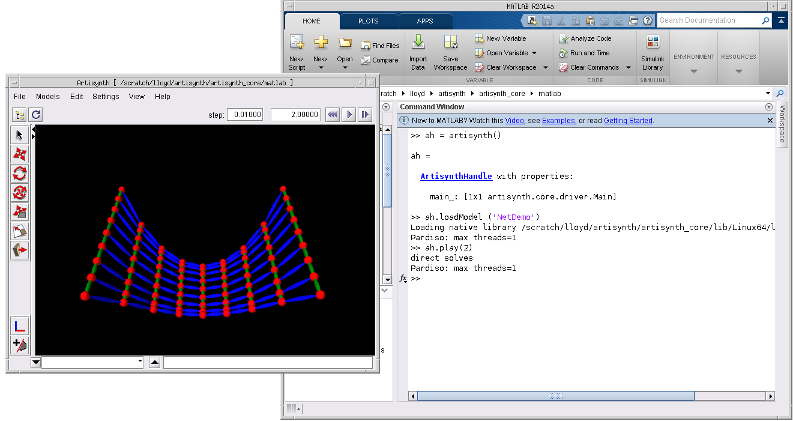
\includegraphics[]{images/artisynthMatlab}
\else
 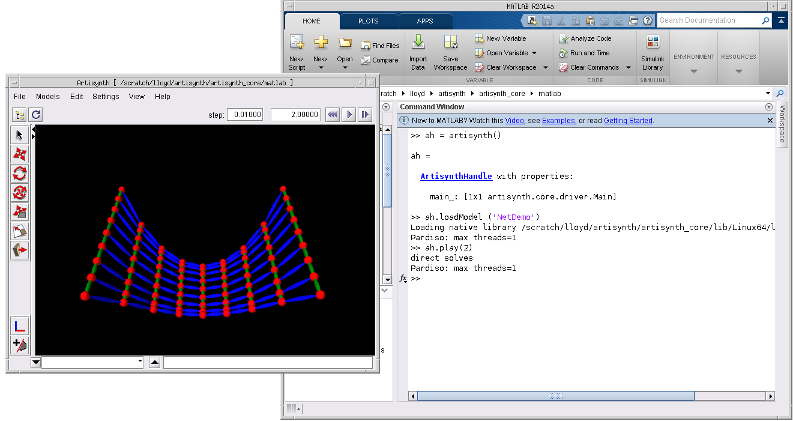
\includegraphics[width=6in]{images/artisynthMatlab}
\fi
\end{center}
\caption{ArtiSynth being run from MATLAB.}
\label{artisynthMatlab:fig}
\end{figure}

If desired, the {\tt artisynth()} command can also accept a variable
length set of strings as arguments, corresponding to the
options available to the {\tt artisynth} terminal command.  For
example,
%
\begin{lstlisting}[]
  >> ah = artisynth('-model', 'SpringMeshDemo')
\end{lstlisting}
%
is equivalent to the terminal command
%
\begin{lstlisting}[]
  > artisynth -model SpringMeshDemo
\end{lstlisting}
%
and causes ArtiSynth to look for and load the model named {\tt
SpringMeshDemo}. However, most of what can be achieved using command
options can also be achieved by directly accessing ArtiSynth
structures or calling handle methods.

%
\begin{sideblock}
Note: at present, if the ArtiSynth GUI is suppressed using the {\tt
-noGui} option, then models must be specified using their fully
qualified class names. For {\tt SpringMeshDemo}, this is {\tt
artisynth.demos.mech.SpringMeshDemo}, and so with the {\tt -noGui}
option the above example would have to be invoked as follows:
%
\begin{verbatim}
   >>> ah = artisynth('-noGui', '-model', 'artisynth.demos.mech.SpringMeshDemo')
\end{verbatim}
%
This is because abbreviated model names are recognized only if
ArtiSynth creates the {\sf Model} menu, which it does not do if the
GUI is not invoked. This restriction may change in future versions of
ArtiSynth.
\end{sideblock}
%

To exit ArtiSynth, you can either select {\sf File > Quit} in the
ArtiSynth GUI, or use the {\tt quit()} method supplied by the handle,
as in
%
\begin{lstlisting}[]
  >> ah.quit()
\end{lstlisting}
%

After quitting, you can use the {\tt artisynth()} command to start
another ArtiSynth session if desired.

\begin{sideblock}
At present, it is not possible to start multiple simultaneous
ArtiSynth instances within MATLAB, although that may change in the
future.
\end{sideblock}

\subsection{Querying ArtiSynth structures and models}
\label{MatlabQuerying:sec}

Through the ArtiSynth handle, it is possible to access most of the
Java objects associated with ArtiSynth and its loaded models.  Public
methods for these objects can be called directly from MATLAB. 
Java objects can be created by calling their constructors
directly, without the need for the keyword {\tt new}.
For example, 
%
\begin{lstlisting}[]
   >> vec = maspack.matrix.Vector3d (1, 2, 3);
\end{lstlisting}
%
creates a new instance of {\tt maspack.matrix.Vector3d} and
initializes it to (1, 2, 3). As in Java, import statements can be used
to allow classes to be specified without using their full package
names:
%
\begin{lstlisting}[]
   >> import maspack.matrix.*
   >>
   >> vec = Vector3d (1, 2, 3);
\end{lstlisting}
%
For more details on working with Java objects inside MATLAB, see {\sf
Call Java Libraries} in the MATLAB documentation.

To easily access particular components of a model, the handle method
{\tt getsel()} provides access to to the ArtiSynth selection
list. That means you can select items in the ArtiSynth GUI (using
either the viewer or navigation panel) and then retrieve these into
MATLAB using {\tt getsel()}. If called with no arguments, {\tt
getsel()} returns the entire selection list as a cell array.  If
called with an integer argument {\tt i}, {\tt getsel(i)} returns the
i-th entry in the selection list (where the index {\tt i} is 1-based).

For example, if two particles are currently selected in ArtiSynth, then
{\tt getsel()} can be used as follows:
%
\begin{lstlisting}[]
   >> ah.getsel()       % get entire selection list
   
   ans = 

       [1x1 artisynth.core.mechmodels.Particle]
       [1x1 artisynth.core.mechmodels.Particle]

   >> ah.getsel(1)      % get first item on the selection list

   artisynth.core.mechmodels.Particle@49752dd4
   
\end{lstlisting}
%
Once a component has been selected, then one has access to all its
public methods. The functions {\tt mmat()}, {\tt amat()}, and {\tt
avec()} can be used to map between MATLAB arrays and ArtiSynth {\tt
Matrix} and {\tt Vector} objects:

\begin{description}

\item[{\tt mmat(obj)}]\mbox{}

Creates a MATLAB array from an ArtiSynth 
\javaclass[maspack.matrix]{Vector} or 
\javaclass[maspack.matrix]{Matrix}
object. If the {\tt Matrix} is an instance of 
\javaclass[maspack.matrix]{SparseMatrix}, then
{\tt mmat()} returns a MATLAB sparse matrix. If {\tt obj} is not a
{\tt Vector} or {\tt Matrix}, then the method returns the empty
matrix.

\item[{\tt amat(M)}]\mbox{}

Creates an ArtiSynth \javaclass[maspack.matrix]{Matrix} from a MATLAB
array: either a \javaclass[maspack.matrix]{MatrixNd} if {\tt M} is a
full matrix, or a \javaclass[maspack.matrix]{SparseMatrixNd} if {\tt
M} is sparse.

\item[{\tt avec(M)}]\mbox{}

Creates an ArtiSynth \javaclass[maspack.matrix]{VectorNd} from a
MATLAB array. At least one of the dimensions of {\tt M} must be 1.

\end{description}

As a simple example, assume that {\tt part} refers to an ArtiSynth
\javaclass[artisynth.core.mechmodels]{Particle}
object. The following code fragment 
then obtains the particle's position as a MATLAB array,
scales it by 3, and then uses this to reset the position:
%
\begin{lstlisting}[]
   >> import maspack.matrix.*
   >> 
   >> pos = mmat(part.getPosition())

   pos =

         5
         0
        10

   >> pos = 3*pos;
   >> part.setPosition (Point3d (avec(pos)));
\end{lstlisting}
%
The particle's position is returned by the method 
\javamethod[artisynth.core.mechmodels.Point]{getPosition()},
which returns a \javaclass[maspack.matrix]{Point3d}. 
Since this is an instance of {\tt
Vector}, we use {\tt mmat()} to turn this into a MATLAB array named {\tt
pos}.  After scaling, we turn this back into an ArtiSynth Vector using
{\tt avec(pos)} and reset the particle's position using the
\javamethod[artisynth.core.mechmodels.Point]{setPosition()}
method. This method requires a {\tt Point3d}
argument, whereas {\tt avec(pos)} returns a more general {\tt
VectorNd} object. However, we can create the required
{\tt Point3d} from the {\tt VectorNd} using the {\tt Point3d(Vector)}
constructor.

As a more complex example, assume that {\tt fem} refers to an
ArtiSynth \javaclass[artisynth.core.femmodels]{FemModel3d}. The
following code fragment then obtains the stiffness matrix for this
model and uses MATLAB to find its largest Eigenvalues:
%
\begin{lstlisting}[]
   >> K = mmat (fem.getActiveStiffness());
   >> eigs (K)
   
   ans =
   
      1.0e+04 *
   
      -8.5443
      -8.5443
      -6.6442
      -6.6442
      -5.0636
      -4.4762
\end{lstlisting}
%
The current stiffness matrix associated with the active nodes is
returned by {\tt getActiveStiffness()}. Since this is an instance of
\javaclass[maspack.matrix]{SparseBlockMatrix}, {\tt mmat()} converts
it to a MATLAB sparse matrix, for which we can then find the largest
Eigenvalues using {\tt eigs()}.

It is also possible to directly query and set the numeric data
associated with ArtiSynth input and output probes. This makes it
possible to use MATLAB to plot or process output probe data, or
compute and prepare input probe data.

Methods to access probe data are provided by the {\tt ArtisynthHandle}:
%
\begin{lstlisting}[]
   getIprobeData (name);     // get data for the specified input probe
   setIprobeData (name, D)   // set data for the specified input probe
   getOprobeData (name)      // get data for the specified output probe
   setOprobeData (name, D)   // set data for the specified output probe
\end{lstlisting}
%
The probe in question must be a {\it numeric probe}, i.e., an instance of 
\javaclass[artisynth.core.probes]{NumericProbeBase}. {\tt
name} is a string giving either the name or number of the probe. The
{\tt get()} methods return the data as a MATLAB array, while the {\tt
set()} methods receive the data as the MATLAB array {\tt D}.  The
data array is $m \times n$, where $m$ is the number of knot points
and $n$ is the size of the probe's data vector.

The following example shows the process of obtaining and then changing
the numeric data for input probe 0 of the model {\tt SpringMeshDemo}:
%
\begin{lstlisting}[]
   >> D = ah.getIprobeData ('0')
   
   D =
   
            0  -10.0000         0   20.0000
       1.0000         0         0   20.0000
       1.9400   10.0000         0    6.8000
       3.0000         0         0   10.0000
       4.0000  -10.0000         0   20.0000
       5.0000         0         0   20.0000
       6.0000   10.0000         0   20.0000
       7.0000         0         0   10.0000
       8.0000  -10.0000         0   20.0000
       9.0000         0         0   20.0000
      10.0000   10.0000         0   20.0000
      11.0000         0         0   10.0000
   
   >> % Now change D by removing all but the first 5 knot points:
   >> D = D(1:5,:);
   >> ah.setIprobeData ('0', D);
\end{lstlisting}
%

\begin{sideblock}
When setting probe data from MATLAB, the number of columns in the
supplied data array must equal the current size of the probe's data
vector.
\end{sideblock}

\subsection{Scripting commands}
\label{MatlabScripting:sec}

The {\tt ArtisynthHandle} object contains a number of methods that
make it possible to load models and control simulation directly from
MATLAB, rather than using the ArtiSynth GUI. A full summary of these
methods is given Section \ref{ScriptingMethods:sec}.

In particular, it is possible to load a model and then run or single
step a simulation.

To load a model, one may use the method
%
\begin{lstlisting}[]
  loadModel (name, args...)
\end{lstlisting}
%
where {\tt name} is either the fully-qualified classname of the
model's 
\javaclass[artisynth.core.workspace]{RootModel},
or one of the shorter names that appears
under the ArtiSynth {\sf Models} menu, and {\tt args...} is an
optional variable-length list of string arguments that are used to
form the {\tt args} argument of the model's {\tt build()} method.

Once loaded, simulation may be controlled using methods such as {\tt
play()}, {\tt pause()}, {\tt step()}, or {\tt reset()}. The following
example shows loading a model called {\tt RigidBodyDemo} and
then having it simulate for 2.5 seconds:
%
\begin{lstlisting}[]
   >> ah.loadModel ('RigidBodyDemo');
   >> ah.play (2.5);
\end{lstlisting}
%
A particularly powerful feature is the ability to single step
execution in a loop, allowing MATLAB to be used to control or inspect
the simulation while it is in progress:
%
\begin{lstlisting}[]
   >> % single step the simulation for 100 steps
   >> for i=1:100
   >>    ... adjust inputs if desired ...
   >>    ah.step();
   >>    ... monitor outputs if desired ...
   >> end
\end{lstlisting}
%
This allows MATLAB code to surround each simulation step, assuming a
role analogous to the \javaclass[artisynth.core.modelbase]{Controller}
or \javaclass[artisynth.core.modelbase]{Monitor} objects that can be
added to the {\tt RootModel}.  The adjustment of inputs or monitoring
of outputs can be accomplished by setting or querying input or output
variables of appropriate model components. One way to obtain access to
these components is through the {\tt find()} method discussed above.
As a simple example, consider the {\tt SimpleMuscleWithController}
demo describe the {\it ArtiSynth Modeling Guide}. The same effect
can be achieved by loading {\tt SimpleMuscle} and then adjusting
target position of point {\tt p1} directly in MATLAB:
%
\begin{lstlisting}[]
   >> import maspack.matrix.Point3d
   >> ah.loadModel ('SimpleMuscle');
   >> p1 = ah.find('models/0/particles/p1');
   >> for i=1:100
   >>    ang = ah.getTime()*pi/2;
   >>    targ = 0.5*[sin(ang), 0, 1-cos(ang)];
   >>    p1.setTargetPosition (Point3d (avec (targ)));
   >>    ah.step();
   >>    pause (0.01); % slow down simulation if desired
   >> end
\end{lstlisting}
%
The call to {\tt pause()} in the above code simply slows down the
simulation so that it appears to run in real time.

\subsection{Java memory limits}
\label{memoryLimits:sec}

ArtiSynth applications often require a large amount of memory,
requiring that the memory limit for the Java virtual machine
be set fairly high (perhaps to several gigabytes). By contrast, the
default Java memory limit set by MATLAB is often much lower, and so it
may be necessary to increase this.

If the memory limit is too low, you may get an out-of-memory error,
which generally produces a stack trace on the MATLAB console along
with an error message of the form
%
\begin{lstlisting}[]
Exception in thread "AWT-EventQueue-0"
java.lang.OutOfMemoryError: Java heap space
\end{lstlisting}
%

The standard way to increase the MATLAB Java memory limit is from the
{\sf Preferences} menu:

{\sf Preferences > MATLAB > General > Java Heap Memory}

MATLAB will need to be restarted for any change of settings to take
effect.

Unfortunately, at the time of this writing, MATLAB limits the maximum
memory size that can be set this way to about 1/4 of the physical
memory on the machine, and lower limits have been reported on some
systems. If you need more memory than the preferences
settings are willing to give you, then you can try creating or editing
the {\tt java.opts} file located in {\tt \$MATLABROOT/bin/\$ARCH},
where {\tt \$MATLABROOT} is the MATLAB installation root directory and
{\tt \$ARCH} is an architecture-specific directory. Within the {\tt
java.opts} file, you can use the {\tt -Xmx} option to increase the
memory limit. As an example, the following {\tt -Xmx} settings
specify memory limits of 128 Mbytes, 2 Gbytes and 4 Gbytes,
respectively:
%
\begin{lstlisting}[]
-Xmx128m 
-Xmx2000m
-Xmx4g
\end{lstlisting}
%
More details are given in
\href{http://www.mathworks.com/support/solutions/en/data/1-18I2C}
{www.mathworks.com/support/solutions/en/data/1-18I2C}.

\subsection{Setting the classpath for ArtiSynth}
\label{ArtisynthClasspath:sec}

Before running ArtiSynth under MATLAB, it is necessary to ensure that
the classes used by ArtiSynth are present within MATLAB's Java
classpath. Letting {\tt <ARTISYNTH\_HOME>} denote the path to the
top-level directory of the ArtiSynth installation, there are
two ways to do this:

\begin{enumerate}

\item Within MATLAB, run the command {\tt setArtisynthClasspath} with
the string associated with {\tt <ARTISYNTH\_HOME>} as an argument.
Assuming the environment variable {\tt ARTISYNTH\_HOME} has been
set, then the following should work:
%
\begin{verbatim}
  >>> setArtisynthClasspath (getenv ('ARTISYNTH_HOME'))
\end{verbatim}
%

\item Create an ASCII text file called {\tt javaclasspath.txt} in one
of the directories in the MATLAB search path, and add to
this the path name for {\tt <ARTISYNTH\_HOME>/classes}, as well as the
path name for each {\tt .jar} file in {\tt <ARTISYNTH\_HOME>/lib}.  So
for example, if {\tt <ARTISYNTH\_HOME>} is {\tt
/home/joe/artisynth\_core}, then the entries in {\tt
javaclasspath.txt} would look like this:
%
\begin{verbatim}
  /home/joe/artisynth_core/classes
  /home/joe/artisynth_core/lib/quickhull3d.jar
  /home/joe/artisynth_core/lib/jython.jar
  /home/joe/artisynth_core/lib/jmf.jar
   ... etc ...
\end{verbatim}
%
For more details on using {\tt javaclasspath.txt}, see\\
\href{https://www.mathworks.com/help/matlab/matlab_external/static-path.html}
{\tt www.mathworks.com/help/matlab/matlab\_external/static-path.html}.

\end{enumerate}

\subsection{Setting the classpath for models}
\label{ModelClasspath:sec}

Usually, ArtiSynth applications involve the use of models or packages
defined outside of the ArtiSynth core. In order for these to be
visible to Java from inside MATLAB, it is necessary to add their
classpaths to MATLAB's Java classpath. There are three ways to do this:

\begin{enumerate}

\item Add the classpaths to the ArtiSynth's external class path.
Instructions for doing this are given the section ``Setting the
external classpath'' of the \artisynthManual{uiguide}{User Interface
Guide}.

\item Add the classpaths within the {\tt MATLAB} session using the
{\tt javaaddpath()} command. This should be done {\it before} the
first call to {\tt artisynth()}, perhaps within a startup script.

\item Add the classpaths to an ASCII text file called {\tt
javaclasspath.txt} located in one of the directories in the MATLAB
search path, as described in Section \ref{ArtisynthClasspath:sec}.

\end{enumerate}

\begin{sideblock}
When adding classpaths for external ArtiSynth models, be sure to add
{\it all} dependencies. For example, if your model resides under {\tt
/home/artisynth\_projects/classes}, but also depends on classes in {\tt
/home/artisynth\_models/classes}, then both of these must be added to
MATLAB's Java classpath.
\end{sideblock}

\begin{sideblock}
Calling {\tt javaaddpath()}
{\it after} the first call to {\tt
artisynth()} may result in some warnings about existing
ArtiSynth classes, such as
\begin{verbatim}
   Warning: Objects of artisynth/core/driver/Main class exist - not clearing java 
   > In javaclasspath>doclear at 377
\end{verbatim}
The added classes may also not be visible to ArtiSynth instances
created by subsequent invocations of {\tt artisynth()}.
\end{sideblock}

\subsection{Connecting to an external MATLAB process}

In addition to being able to run ArtiSynth from within MATLAB, it is
also possible to create a connection between ArtiSynth and an
externally running MATLAB program. Data can then be passed back and
forth between ArtiSynth and MATLAB. This can be particularly useful if
it turns out to be unfeasible to run ArtiSynth directly under MATLAB.

\begin{sideblock}
Caveat: The MATLAB connection uses the
\href{https://code.google.com/p/matlabcontrol}{matlabcontrol}
interface, by Joshua Kaplan. It relies on the undocumented
\href{https://code.google.com/p/wiki/JMI}{Java MATLAB Interface}, and
hence cannot be guaranteed to work with future versions of MATLAB.
\end{sideblock}

An external MATLAB connection can be opened in any of the following
ways:

\begin{enumerate}

\item Choosing {\sf File > Open MATLAB Connection} in the GUI;

\item Specifying the option {\tt -openMatlabConnection} on
the command line;

\item Calling the {\tt openMatlabConnection()} method in the {\tt
Main} class (see Section \ref{MatlabFromCode:sec}).

\end{enumerate}

\begin{sideblock}
When a MATLAB connection is requested, the system will first attempt
to connect to a MATLAB process running on the user's machine. If no
zsuch process is found, then a new MATLAB process will be started.  If
a MATLAB connection is opened when ArtiSynth is being run under
MATLAB, then the connection will be made to the parent MATLAB process.
\end{sideblock}

Once a connection is open, it is possible to save/load probe data
to/from MATLAB. This can be done by selecting the probe and then
choosing either {\sf Save to MATLAB} or {\tt Load from MATLAB} in the
right-click context menu. This will cause the probe data to be saved
to (or loaded from) a MATLAB array. The name of the MATLAB array is
determined by {\tt NumericProbeBase.getMatlabName()}, which returns
either

\begin{enumerate}

\item The name of the probe, if not {\tt null}, or

\item {\tt "iprobe<n>"} (for input probes) or {\tt "oprobe<n>"} (for
output probes), where {\tt <n>} is the probe number.

\end{enumerate}

It is also possible to save/load probe data to/from MATLAB using the
following functions available in ArtiSynth's Jython interface (see the
section ``Jython Interaction and Scripting'' in the
\artisynthManual{uiguide}{User Interface Guide}):
%
\begin{lstlisting}[]
   iprobeToMatlab (probeName, matlabName)
   iprobeFromMatlab (probeName, matlabName)
   iprobeToMatlab (probeName)
   iprobeFromMatlab (probeName)

   oprobeToMatlab (probeName, matlabName)
   oprobeFromMatlab (probeName, matlabName)
   oprobeToMatlab (probeName)
   oprobeFromMatlab (probeName)
\end{lstlisting}
%
{\tt iprobeToMatlab()} and {\tt iprobeFromMatlab()}
save/load data for the input probe specified by {\tt probeName}
to/from the MATLAB variable with the name {\tt matlabName}. {\tt
probeName} is a string giving either the probe's name or number.  If
{\tt matlabName} is absent, then the value of {\tt
NumericProbeBase.getMatlabName()} (described above) is used.  The
functions {\tt oprobeToMatlab()} and {\tt oprobeFromMatlab()} do the
same thing for output probes.

\subsection{Managing an external MATLAB connection from code}
\label{MatlabFromCode:sec}

The MATLAB connection is associated, internally, with a structure
called \javaclass[artisynth.core.util]{MatlabInterface}, which
provides the internal methods for sending data to and from MATLAB.
The interface can be obtained and queried from methods in the {\tt
Main} class:

\begin{description}

\item[{\tt MatlabInterface openMatlabConnection()}] \mbox{}

Returns a connection to a MATLAB process. If a connection already
exists, that connection is returned. Otherwise, a new connection is
established with a MATLAB process running on the user's machine.  If
no such process is found, then a new MATLAB process will be
started. If ArtiSynth is being run under MATLAB, then the connection
will be made to the parent MATLAB process

\item[{\tt MatlabInterface getMatlabConnection()}] \mbox{}

Returns the current MATLAB connection, if any; otherwise, returns {\tt
null}.

\item[{\tt boolean hasMatlabConnection()}] \mbox{}

Returns {\tt true} if a MATLAB connection currently exists.

\item[{\tt boolean closeMatlabConnection()}] \mbox{}

Closes any current MATLAB connection, returning {\tt true} if a
connection previously existed.

\end{description}

Methods by which a MatlabConnection can send data to and from MATLAB
include:

\begin{description}

\item[{\tt void objectToMatlab (obj, matlabName)} ] \mbox{}

Sets the MATLAB array named {\tt matlabName} to the values associated
with the ArtiSynth object {\tt obj}. The ArtiSynth object must be
either a \javaclass[maspack.matrix]{Matrix},
\javaclass[maspack.matrix]{Vector}, or {\tt double[][]}.  The assigned MATLAB
array is dense, unless the ArtiSynth object is an instance of
\javaclass[maspack.matrix]{SparseMatrix}, in which the array
is sparse.

\item[{\tt double[][] arrayFromMatlab (matlabName)}] \mbox{}

Takes the MATLAB array named by {\tt matlabName} and returns the
corresponding {\tt double[][]} object, with values assigned in
row-major order. If the named MATLAB array does not exist, or is not
dense and 2-dimensional, then {\tt null} is returned.

\item[{\tt Matrix matrixFromMatlab (matlabName)}] \mbox{}

Takes the MATLAB array named by {\tt matlabName} and returns a
corresponding \javaclass[maspack.matrix]{Matrix} object.  If the named
MATLAB array does not exist, or is not 2-dimensional, then {\tt null}
is returned. Otherwise, either a \javaclass[maspack.matrix]{MatrixNd}
or \javaclass[maspack.matrix]{SparseMatrixNd} is returned, depending
on whether the array is dense or sparse.

\item[{\tt Matrix matrixFromMatlab (matlabName)}] \mbox{}

Takes the MATLAB array named by {\tt matlabName} and returns a
corresponding \javaclass[maspack.matrix]{VectorNd} object.  If the
named MATLAB array does not exist, or is not 2-dimensional with a size
of 1 in at least one dimension, then {\tt null} is returned.

\end{description}

The above methods are also available in the Jython interface (
(section ``Jython Interaction and Scripting'' of the
\artisynthManual{uiguide}{User Interface Guide}) via the functions
%
\begin{lstlisting}[]
   objectToMatlab (obj, matlabName)
   arrayFromMatlab (matlabName)
   matrixFromMatlab (matlabName)
   vectorFromMatlab (matlabName)
\end{lstlisting}
%

The following example shows a code fragment in which a MATLAB
connection is obtained and then used to transfer data to and from
MATLAB:

\begin{lstlisting}
   import artisynth.core.driver.Main;
   import artisynth.core.util.MatlabInterface;

   ...

   Main main = Main.getMain();
   MatlabInterface mi = main.openMatlabConnection();

   // read a matrix MX from MATLAB. Assume we know a-priori that
   // MX is dense, so it will be returned as a MatrixNd
   MatrixNd MX = (MatrixNd)mi.matrixFromMatlab ("MX");

   // send a sparse matrix K to MATLAB and assign it the name KMAT
   SparseMatrix K = ...
   mi.objectToMatlab (K, "KMAT");
\end{lstlisting}


\section{Summary of scripting functions}
\label{ScriptingMethods:sec}

The following is a summary of the scripting functions available
in MATLAB through the {\tt ArtisynthHandle} object:

\begin{description}

\item[{\tt getMain()}] \mbox{}

Returns the ArtiSynth {\tt Main} object.

\item[{\tt loadModel (name, args...)}] \mbox{}

Loads the named model along with optional arguments.  {\tt name} is
the classname of the model's
\javaclass[artisynth.core.workspace]{RootModel} and {\tt args...} is
an optional variable-length list of string arguments that are used to
form the {\tt args} argument of the model's {\tt build()} method.
Nominally, {\tt name} should be a fully-qualified classname (e.g.,
{\tt artisynth.demos.mech.RigidBodyDemo}), but if the model has been
loaded before, the simple class name should work as well (e.g., {\tt
RigidBodyDemo}).

\item[{\tt loadModelFile (filename)}] \mbox{}

Loads a model from an ArtiSynth file. {\tt filename} is a string
giving the file's path.

\item[{\tt saveModelFile (filename)}] \mbox{}

Save a model to an ArtiSynth file.

\item[{\tt saveModelFile (filename, saveWayPointData, coreCompsOnly)}] \mbox{}

Save a model to an ArtiSynth file. The options {\tt saveWayPointData}
and {\tt coreCompsOnly} specify whether to (a) save waypoint data, and
(b) save only components from {\tt artisynth\_core}.

\item[{\tt play()}] \mbox{}

Starts the simulation running.

\item[{\tt play(t)}] \mbox{}

Starts and runs the simulation for {\tt t} seconds.

\item[{\tt pause()}] \mbox{}

Pauses the simulation.

\item[{\tt step()}] \mbox{}

Single steps the simulation.

\item[{\tt reset()}] \mbox{}

Resets the simulation to time 0.

\item[{\tt forward()}] \mbox{}

Forwards the simulation to the next waypoint.

\item[{\tt rewind()}] \mbox{}

Rewinds the simulation to the last waypoint.

\item[{\tt delay(t)}] \mbox{}

Delays execution for {\tt t} seconds. In MATLAB, the same effect can
be achieved using the MATLAB command {\tt pause(t)}.

\item[{\tt waitForStop()}] \mbox{}

Blocks until the simulation has completed.

\item[{\tt isPlaying()}] \mbox{}

Returns {\tt true} if simulation is still running.

\item[{\tt getTime()}] \mbox{}

Returns current ArtiSynth simulation time in seconds.

\item[{\tt reload()}] \mbox{}

Reloads the current model.

\item[{\tt addWayPoint(t)}] \mbox{}

Adds a simulation waypoint at time {\tt t},
where {\tt t} is a floating point value giving
the time in seconds.

\item[{\tt addBreakPoint(t)}] \mbox{}

Adds a breakpoint at time {\tt t}.

\item[{\tt removeWayPoint(t)}] \mbox{}

Removes any waypoint or breakpoint at time {\tt t}.

\item[{\tt clearWayPoints()}] \mbox{}

Removes all waypoints and breakpoints.

\item[{\tt saveWayPoints (filename)}] \mbox{}

Save waypoints and their data to a specified file

\item[{\tt loadWayPoints (fileName)}] \mbox{}

Load waypoints and their data from a specified file

\item[{\tt root()}] \mbox{}

Returns the current RootModel.

\item[{\tt find (path)}] \mbox{}

Finds a component defined by {\tt path} with respect to the current RootModel.

\item[{\tt getsel()}] \mbox{}

Returns the current ArtiSynth selection list.

\item[{\tt getsel(i)}] \mbox{}

Returns the i-th selection list item (1-based for MATLAB).

\item[{\tt quit()}] \mbox{}

Quits ArtiSynth.

\end{description}

\end{document}
